\chapter{宏}\label{ch21}

\emph{A cento (from the Latin for “patchwork”) is a poem made up entirely of lines quoted from another poet.}
\begin{flushright}
    ——Matt Madden
\end{flushright}

Rust支持\emph{宏(macros)}:一种普通函数无法做到的扩展语言的方式。例如,我们已经看到过\texttt{assert\_eq!}宏,它可以方便地用来测试:
\begin{minted}{Rust}
    assert_eq!(gcd(6, 10), 2);
\end{minted}

这也可以写成一个泛型函数,但\texttt{assert\_eq!}可以做到几件函数做不到的事。一是当断言失败时,\texttt{assert\_eq!}会生成包含断言所在的文件名和行号的错误消息。函数没有办法获得这些信息。但宏可以,因为它们工作的方式完全不同。

宏是一种缩写。在编译期间,在类型检查之前、更在生成任何机器码之前,每一个宏调用都会被\emph{展开(expand)}——即,被替换为一些Rust代码。上面的宏调用会展开成类似这样的代码:
\begin{minted}{Rust}
    match (&gcd(6, 10), &2) {
        (left_val, right_val) => {
            if !(*left_val == *right_val) {
                panic!("assertion failed: `(left == right)`, \
                        (left: `{:?}`, right: `{:?}`)", left_val, right_val));
            }
        }
    }
\end{minted}

\texttt{panic!}也是一个宏,它自己会展开成更多Rust代码(这里没有展示)。那些代码里用到了两个别的宏,\texttt{file!()}和\texttt{line!()}。一旦crate中的每一个宏调用都被完全展开,Rust会进入编译的下一个阶段。

在运行时,一个断言失败看起来像这样(并且可能指示\texttt{gcd()}函数中的一个bug,因为\texttt{2}是正确的答案):
\begin{minted}{text}
    thread 'main' panicked at 'assertion failed: `(left == right)`, (left: `17`,
    right: `2`)', gcd.rs:7
\end{minted}

如果你是从C++来的,你可能经历过一些宏的糟糕体验。Rust的宏采用了一种不同的方式,类似于Scheme的\texttt{syntax-rules}。相比于C++的宏,Rust的宏和语言的其他部分集成得更好,并且因此更不容易出错。宏调用总是用感叹号标记,这样当你阅读代码时它们会很显眼,并且不会在你想调用函数时偶然错误地调用成了宏。Rust的宏从来不会插入不匹配的花括号或圆括号。并且Rust的宏带有模式匹配,这使得编写既可维护又易于使用的宏变得更容易。

在本章中,我们将通过几个简单的示例展示如何编写宏。但和Rust中的很多部分一样,宏值得深入理解,所以我们将介绍一个更复杂的宏的设计,它允许我们直接在我们的程序中嵌入JSON字面量。但除了本书中介绍的部分之外,宏还有更多的内容。因此我们将以一些进一步学习的点结束,既有我们将在这里向你展示的高级技巧,也有功能更加强大的设施称为\emph{过程宏(procedural macros)}。

\section{宏基础}
\autoref{f21-1}展示了\texttt{assert\_eq!}宏的部分源码。

\begin{figure}[htbp]
    \centering
    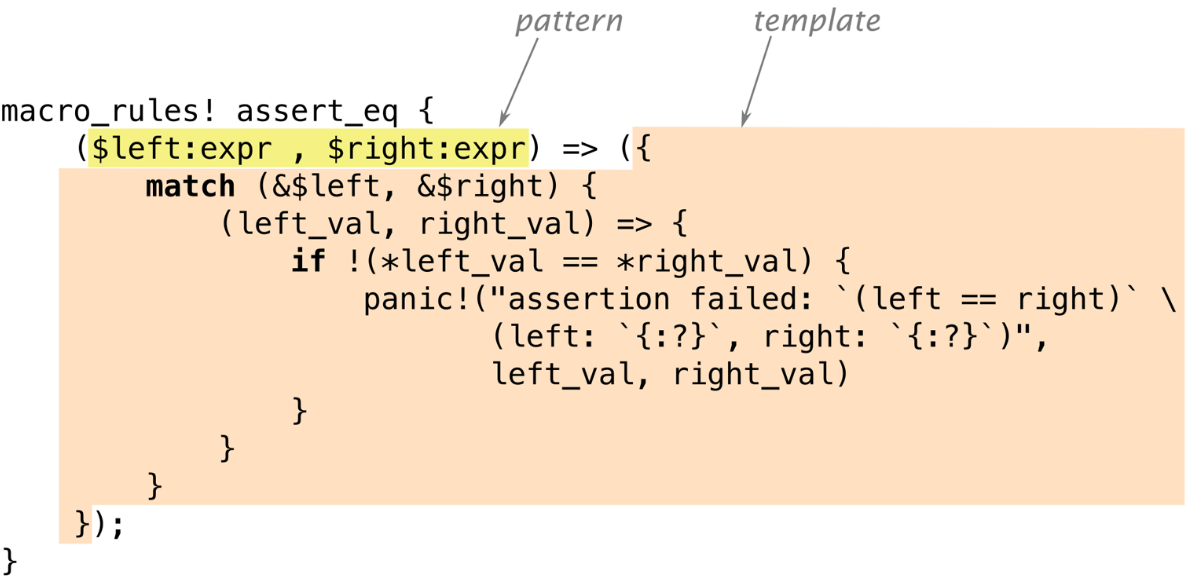
\includegraphics[width=0.9\textwidth]{../img/f21-1.png}
    \caption{\texttt{assert\_eq!}宏}
    \label{f21-1}
\end{figure}

\texttt{macro\_rules!}是Rust中定义宏的主要方法。注意,宏定义里\texttt{assert\_eq}后边没有\texttt{!}:只有在调用宏时才需要\texttt{!},定义时不需要。

并不是所有的宏都是以这种方式定义的:少数的宏,例如\texttt{file!}、\texttt{line!}和\texttt{macro\_rules!}自身,是编译器内建的。我们将在本章的末尾讨论另一种方法,称为过程宏。但我们的主要精力还是集中在\texttt{macro\_rules!},这是(目前为止)最容易的编写自己的宏的方法。

一个用\texttt{macro\_rules!}定义的宏完全靠模式匹配工作。宏的主体只是一系列规则:
\begin{minted}{text}
    ( pattern1 ) => ( template1 );
    ( pattern2 ) => ( template2 );
    ...
\end{minted}

\autoref{f21-1}中的\texttt{assert\_eq!}版本只有一个模式和一个模板。

顺便,你可以使用方括号或者花括号来代替模式或模板两侧的圆括号,对Rust来说它们并没有任何区别。另外,当你调用一个宏时,这些都是等价的:
\begin{minted}{Rust}
    assert_eq!(gcd(6, 10), 2);
    assert_eq![gcd(6, 10), 2];
    assert_eq!{gcd(6, 10), 2}
\end{minted}

唯一的不同是花括号后边的分号是可选的。为了方便,我们在调用\texttt{assert\_eq!}时使用圆括号,调用\texttt{vec!}时使用方括号,\texttt{macro\_rules!}时使用花括号。

现在我们展示了一个宏展开的简单示例和生成这个宏的定义,我们可以深入了解它工作的细节:
\begin{itemize}
    \item 我们将详细地解释Rust是怎么发现和展开你的程序中的宏定义的。
    \item 我们将指出在根据宏模板生成代码时的一些细节之处。
    \item 最后,我们将展示模式如何处理重复的结构。
\end{itemize}

\subsection{宏展开基础}
Rust会在编译的前期展开宏。编译器会从头到尾读取源码,在这个过程中定义和展开宏。宏只有在定义之后才能被调用,因为Rust会立刻展开每一个宏调用,而不会去看程序的剩余部分。(相反,函数和其他的\hyperref[static]{item}的定义不需要按照任何顺序。调用一个后面才定义的函数也是OK的。

当Rust展开一个\texttt{assert\_eq!}宏调用时,行为和执行一个\texttt{match}表达式非常像。Rust首先根据模式匹配参数,如\autoref{f21-2}所示:
\begin{figure}[htbp]
    \centering
    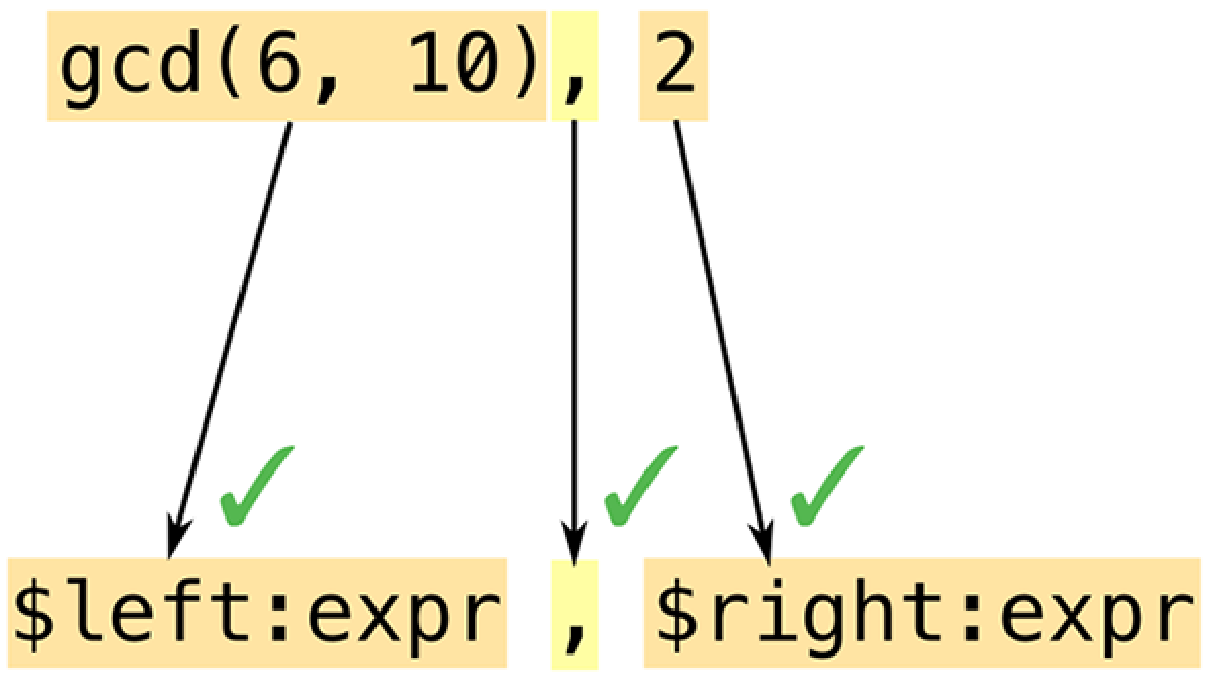
\includegraphics[width=0.8\textwidth]{../img/f21-2.png}
    \caption{展开一个宏,第1部分:用模式匹配参数}
    \label{f21-2}
\end{figure}

宏的模式是Rust的mini语言。它们本质上是匹配代码的正则表达式。但普通的正则表达式是操作字符,而模式操作\emph{token(词元)}——数字、变量名、标点符号等Rust中的构建块。这意味着你可以在宏模式中自由地使用注释和空格来提升它们的可读性。注释和空格不是token,因此它们不会影响到匹配。

正则表达式和宏模式的另一个重要不同之处是圆括号、方括号、花括号在Rust中总是成对出现。这一点会在宏展开之前就检查,不仅仅是在宏模式中,而且是在整个语言中。

在这个例子中,我们的模式包含了\emph{fragment(片段)} \texttt{\$left:expr},这告诉Rust去匹配一个表达式(在这个例子中,就是\texttt{gcd(6, 10)}并把它复制到名称\texttt{\$left}。然后Rust用\texttt{gcd}调用后边的逗号匹配模式中的逗号。类似于正则表达式,模式只有少数特殊字符会触发有趣的匹配行为;其它的所有字符,例如逗号,都必须逐字匹配相同的字符,否则就会匹配失败。

这个模式中的两个代码片段都是\texttt{expr}类型:它们代表表达式。我们将在“\nameref{FragType}”中看到其他类型的代码片段。

因为这个模式匹配到了所有的参数,Rust会展开相应的\emph{template(模板)}(\autoref{f21-3}):
\begin{figure}[htbp]
    \centering
    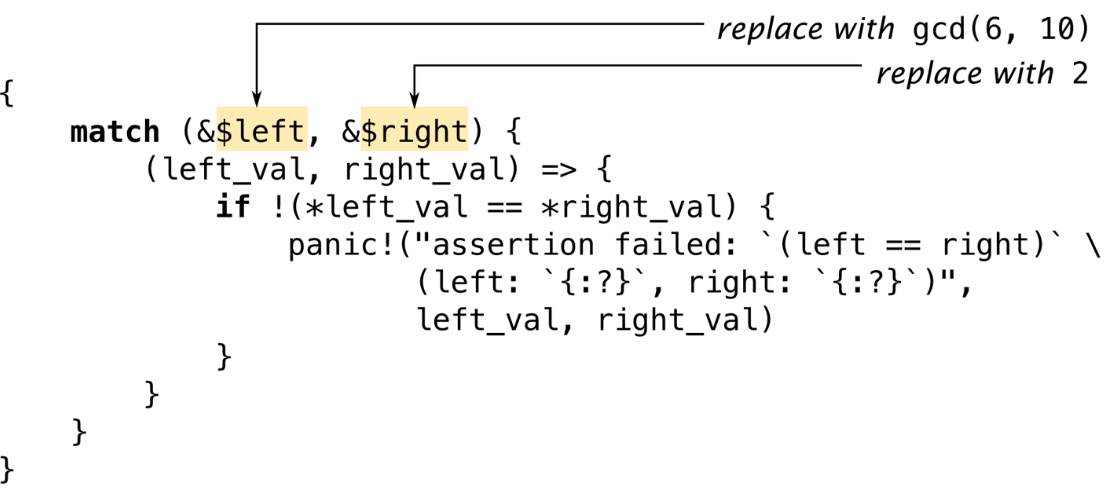
\includegraphics[width=0.9\textwidth]{../img/f21-3.png}
    \caption{展开一个宏,第2部分:填充模板}
    \label{f21-3}
\end{figure}

Rust会用匹配阶段发现的代码片段来替换\texttt{\$left}和\texttt{\$right}。

一个常见的错误是在输出模板中包含片段的类型:写\texttt{\$left:expr}而不是\texttt{\$left}。Rust不会立刻检测出这种错误。它会把\texttt{\$left}看错一个整体,然后把\texttt{:expr}看作和模板中其他部分一样的东西:要包含在宏的输出中的词元。因此只有当你\emph{调用}这个宏时这个错误才会出现;然后它会生成错误的不能编译的输出。如果你在使用一个新的宏时得到了类似\texttt{cannot find type `expr` in this scope}和\texttt{help: maybe you meant to use a path separator here}这样的错误消息,可以检查下它是不是有这个错误。(“\nameref{DebugMacro}”提供了更多类似这种情况的建议。)

宏模板和web编程中常用的很多种模板语言中的任意一种都没有太大的区别。唯一的不同——也是很重要的一点——就是它的输出是Rust代码。

\subsection{意外的结果}
把代码片段插入模板和普通的处理值的代码有一些区别。这些区别一开始可能并不明显。我们之前看到的\texttt{assert\_eq!}宏包含了一些有些奇怪的代码,这是宏编程特有的。让我们重点看看其中两个有趣的部分。

首先,为什么这个宏创建了两个变量\texttt{left\_val}和\texttt{right\_val}?为什么我们不能把模板简化成这样?
\begin{minted}{Rust}
    if !($left == $right) {
        panic!("assertion failed: `(left == right)` \
                (left: `{:?}`, right: `{:?}`)", $left, $right)
    }
\end{minted}
为了回答这个问题,尝试手动展开宏调用\texttt{assert\_eq!(letters.pop(), Some('z'))}。输出将会是什么?Rust会把匹配到的表达式插入模板中的多个位置。看起来在构建错误消息时重新求值表达式是一个坏主意,原因不仅仅是因为它需要消耗两倍的时间:因为\texttt{letters.pop()}从vector中移除一个值,所以在我们第二次调用它时会产生一个和第一次不同的值!这就是为什么真正的宏只计算一次\texttt{\$left}和\texttt{\$right},然后存储它们的值。

来到第二个问题:为什么这个宏借用了\texttt{\$left}和\texttt{\$right}的值的引用?为什么不直接把它们的\emph{值}存进变量中,像这样?
\begin{minted}{Rust}
    macro_rules! bad_assert_eq {
        ($left:expr, $right:expr) => ({
            match ($left, $right) {
                (left_val, right_val) => {
                    if !(left_val == right_val) {
                        panic!("assertion failed" /* ... */);
                    }
                }
            }
        });
    }
\end{minted}

对于我们展示过的特殊情况,即宏的参数是整数的情况下,这可以正常工作。但如果调用者传递了一个\texttt{String}变量作为\texttt{\$left}或\texttt{\$right},这段代码将会移动变量的值!
\begin{minted}{Rust}
    fn main() {
        let s = "a rose".to_string();
        bad_assert_eq!(s, "a rose");
        println!("confirmed: {} is a rose", s);    // error: use of moved value "s"
    }
\end{minted}

因为我们不想让断言移动值,所以宏里使用了引用。

(你可能想知道为什么这个宏使用了\texttt{match}而不是\texttt{let}来定义变量。我们也想知道。事实证明并没有特殊的原因这么做。\texttt{let}是等价的。)

简而言之,宏可能做出令人惊讶的行为。如果一个你写的宏附近发生了奇怪的事,那很可能是这个宏有问题。

C++里的这个经典bug你\emph{将不会}看到:
\begin{minted}{Rust}
    // buggy C++ macro to add 1 to a number
    #define ADD_ONE(n) n + 1
\end{minted}

原因大部分的C++程序员应该很熟悉了,并且不值得详细解释,类似\texttt{ADD\_ONE(1) * 10}或者\texttt{ADD\_ONE(1 << 4)}这样的代码可能会产生令人惊讶的行为。为了修复它,你需要在宏定义中加上更多括号。这在Rust中是不必要的,因为Rust宏和语言集成的更好。Rust知道它什么时候是在处理表达式,因此在把一个表达式粘贴到另一个地方时它会自动添加括号。

\subsection{重复}
标准的\texttt{vec!}宏有两种形式:
\begin{minted}{Rust}
    // 重复一个值N次
    let buffer = vec![0_u8; 1000];

    // 一个逗号分隔的值的列表
    let numbers = vec!["udon", "ramen", "soba"];
\end{minted}

它可以像这样实现:
\begin{minted}{Rust}
    macro_rules! vec {
        ($elem:expr ; $n:expr) => {
            ::std::vec::from_elem($elem, $n)
        };
        ( $( $x:expr ),* ) => {
            <[_]>::into_vec(Box::new([ $( $x ),* ]))
        };
        ( $( $x:expr ),+ ,) => {
            vec![ $( $x ),* ]
        };
    }
\end{minted}

这里有三个规则。我们将解释多个规则是如何工作的,然后依次看看每一个规则。

当Rust展开一个例如\texttt{vec![1, 2, 3]}的宏调用时,它首先尝试匹配参数\texttt{1, 2, 3}和第一条规则的模式,即\texttt{\$elem:expr ; \$n:expr}。这会匹配失败:\texttt{1}是一个表达式,但这个模式要求它后边有一个分号,然而并没有。因此Rust会移动到第二个规则,等等。如果没有规则可以匹配,就会报错。

第一个规则处理类似\texttt{vec![0u8; 1000]}这样的调用。恰好有一个标准(但不在文档里的)函数\texttt{std::vec::from\_elem},正好可以完成我们需要的功能,因此这个规则很直观。

第二个规则处理\texttt{vec!["udon", "ramen", "soba"]}。模式\texttt{\$( \$x:expr ),*}使用了一个我们之前没有提过的的特性:重复。它匹配0个或多个逗号分隔的表达式。更一般地来说,语法\texttt{\$( PATTERN ),*}用来匹配任意逗号分割的列表,其中列表中的每一项匹配\texttt{PATTERN}。

这里的\texttt{*}和正则表达式中的\texttt{*}有相同的含义(“0次或多次”),尽管正则表达式没有特殊的\texttt{,*}重复器。你也可以用\texttt{+}来要求至少一次匹配,或者用\texttt{?}要求0次或1次匹配。\autoref{t21-1}列出了全套的重复模式。

\begin{table}[htbp]
    \centering
    \caption{重复模式}
    \label{t21-1}
    \begin{tabular}{ll}
        \hline
        \textbf{模式} & \textbf{含义} \\
        \hline
        \texttt{\$( ... )*}     & 匹配0次或多次,无分隔符   \\
        \rowcolor{tablecolor}
        \texttt{\$( ... ),*}    & 匹配0次或多次,逗号分隔   \\
        \texttt{\$( ... );*}    & 匹配0次或多次,分号分隔   \\
        \rowcolor{tablecolor}
        \texttt{\$( ... )+}     & 匹配1次或多次,无分隔符   \\
        \texttt{\$( ... ),+}    & 匹配1次或多次,逗号分隔   \\
        \rowcolor{tablecolor}
        \texttt{\$( ... );+}    & 匹配1次或多次,分号分隔   \\
        \texttt{\$( ... )?}     & 匹配0次或1次,无分隔符    \\
        \rowcolor{tablecolor}
        \texttt{\$( ... ),?}    & 匹配0次或1次,逗号分隔    \\
        \texttt{\$( ... );?}    & 匹配0次或1次,分号分隔    \\
    \end{tabular}
\end{table}

代码片段\texttt{\$x}不是单个表达式,而是一个表达式的列表。这个规则的模板也使用了重复语法:
\begin{minted}{Rust}
    <[_]>::into_vec(Box::new([ $( $x ),* ]))
\end{minted}

再一次,恰好有标准方法可以满足我们的需要。这段代码创建了一个装箱的数组,然后使用\texttt{[T]::into\_vec}方法把这个装箱的数组转换成一个vector。

开头的\texttt{<[\_]>},是一种不常见的写法,它表示类型“某些东西的切片”,由Rust来推断元素类型。名字是普通标识符的类型可以直接在表达式中使用,但类似\texttt{fn()}、\texttt{\&str},或者\texttt{[\_]}这样的类型必须用尖括号包裹。

重复模式出现在模板的末尾,即\texttt{\$(\$x),*}。这个\texttt{\$(...),*}和我们在模式中看到的是相同的语法。它迭代\texttt{\$x}匹配到的表达式列表并把它们全部插入模板,用逗号分隔。

在这种情况下看,重复的输出看起来和输入一样。但并不总是这样。我们可以编写类似这样的规则:
\begin{minted}{Rust}
    ( $( $x:expr ),* ) => {
        {
            let mut v = Vec::new();
            $( v.push($x); )*
            v
        }
    };
\end{minted}

这里,模板中\texttt{\$( v.push(\$x); )*}这一部分会对\texttt{\$x}中的每个表达式插入一个\texttt{v.push()}调用。一个宏分支可以展开成一个表达式序列,但这里我们只需要单个表达式,所以我们把vector的处理包装在一个块中。

和Rust中其他部分不同,使用\texttt{\$( ... ),*}并不能自动支持可选的尾部逗号。然而,有一种标准的技巧是通过添加一个额外的规则来支持尾部逗号。也就是我们的\texttt{vec!}宏的第三条规则所做的:
\begin{minted}{Rust}
    ( $( $x:expr ),+ ,) => {    // 如果存在尾部的逗号,
        vec![ $( $x ),* ]       // 重试没有它的情况
    }
\end{minted}

我们使用\texttt{\$( ... ),+ ,}来匹配一个有额外逗号的列表。然后,我们在模板中递归调用了\texttt{vec!},但排除了那个逗号。这一次第二条规则将会匹配。

\section{内建的宏}
Rust编译器提供了几个宏,如果你要定义自己的宏,它们可能会发挥作用。这些宏都不能使用\texttt{macro\_rules!}来实现。它们被硬编码进\texttt{rustc}:

\codeentry{file!(), line!(), column!()}

\hangparagraph{\texttt{file!()}展开成一个字符串字面量:当前的文件名。\texttt{line!()}和\texttt{column!()}展开成\texttt{u32}字面量,表示当前的行号和列号(从1开始计数)。}

\hangparagraph{如果一个宏调用了另一个宏,那个宏又调用了另一个宏,这三个宏在不同的文件中,并且最后一个宏调用了\texttt{file!(), line!()}或者\texttt{column!()},它会展开成\emph{第一个}宏调用的位置。}

\codeentry{stringify!(...tokens...)}

\hangparagraph{展开成一个包含给定token的字符串字面量。\texttt{assert!}宏就是使用了它来生成一条包含了断言代码的错误信息。}

\hangparagraph{参数中的宏调用\emph{不会}被展开:\texttt{stringify!(line!())}会展开为\texttt{"line!()"}。}

\hangparagraph{Rust根据token构建字符串,因此生成的字符串里没有换行符或者注释。}

\codeentry{concat!(str0, str1, ...)}

\hangparagraph{连接参数开展为单个字符串字面量。}

Rust还定义了下面这些宏用来查询构建环境:

\codeentry{cfg!(...)}

\hangparagraph{展开为一个bool常量,如果当前的构建环境满足括号里的条件则为\texttt{true}。例如,如果在编译时启用了调试断言那么\texttt{cfg!(debug\_assertions)}为真。}

\hangparagraph{这个宏和\nameref{attribute}中介绍过的\texttt{\#[cfg(...)]}属性的语法完全相同,但它不是条件编译,而是得到一个true或者false。}

\codeentry{env!("VAR\_NAME")}

\hangparagraph{展开为一个字符串:在编译时该环境变量的值。如果这个变量不存在,会产生编译错误。}

\hangparagraph{除了Cargo在编译crate时设置的几个有趣的环境变量之外,这个宏毫无价值。例如,为了得到crate当前的版本,你可以写:}
\begin{minted}{Rust}
        let version = env!("CARGO_PKG_VERSION");
\end{minted}

\hangparagraph{这些环境变量的完整列表见\href{https://doc.rust-lang.org/cargo/reference/environment-variables.html\#environment-variables-cargo-sets-for-crates}{Cargo文档}。}

\codeentry{option\_env!("VAR\_NAME")}

\hangparagraph{它和\texttt{env!}宏一样,除了它返回一个\texttt{Option<\&'static str>},当环境变量没有设置时返回\texttt{None}。}

还有更多内建的宏可以让你引入另一个文件中的代码或者数据:
\codeentry{include!("file.rs")}

\hangparagraph{展开为指定文件的内容,必须是有效的Rust代码——表达式或者\hyperref[declaration]{item}的序列。}

\codeentry{include\_str!("file.txt")}

\hangparagraph{展开成一个包含指定文件内容的\texttt{\&'static str}。你可以像这样使用它:}

\begin{minted}{Rust}
        const COMPOSITOR_SHADER: &str =
            include_str!("../resources/compositor.glsl");
\end{minted}

\hangparagraph{如果文件不存在或者不是有效的UTF-8,会产生编译错误。}

\codeentry{include\_bytes!("file.dat")}

\hangparagraph{和上一个基本相同,除了它把文件当作二进制数据而不是UTF-8文本,结果是一个\texttt{\&'static [u8]}。}

和所有的宏一样,这些宏也是在编译时进行处理。如果文件不存在或者不能被读取,就会编译失败。它们不可能在运行时出错。在任何情况下,如果文件名是一个相对路径,它会被解析为相对于当前文件所在的目录的路径。

Rust还提供了几个方便的宏:
\codeentry{todo!(), unimplemented!()}

\hangparagraph{这些等价于\texttt{panic!()},但用于表示不同的意图。\texttt{unimplemented!()}出现在\texttt{if}分支、\texttt{march}分支,以及其它还未处理的case中。它总是会panic。\texttt{todo!()}大致相同,但传达的意图是代码还没写完;一些IDE使用它来进行标记。}

\codeentry{matches!(value, pattern)}

\hangparagraph{比较一个值和一个模式,当它们匹配时返回\texttt{true},否则返回\texttt{false}。它等价于写:}

\begin{minted}{Rust}
        match value {
            pattern => true,
            _ => false
        }
\end{minted}

\hangparagraph{如果你在寻找基本的编写宏的练习,这是一个很好的例子——尤其是你可以在标准库文档中看到它的实际实现非常简单。}

\section{调试宏}\label{DebugMacro}


\section{构建\texttt{json!}宏}


\subsection{片段类型}\label{FragType}
